The objective of this work is to coordinate material-handling missions through a progressive workload assignment strategy, while preserving each order as an indivisible unit owned by the resource. The reference configuration consists of eight operational resources, each composed of a human operator and the corresponding forklift. All orders are assumed to be known at the beginning of the simulation.\footnote{Orders could instead become available progressively during the working day if the dataset were provided online. For the sake of the problem, in the present implementation all data are read at the beginning of the program.}

The adopted policy organizes execution into global batches, each characterized by a target of \(x\) completed missions. Failed missions do not contribute to the main objective, whereas missions that have already been admitted or are currently being executed reserve the corresponding available slots. Each resource is assigned a short queue, whose size is limited both by the number of missions and by the expected temporal workload. When a queue is exhausted, the scheduler may replenish it by giving priority to the remaining missions belonging to orders that have already been assigned. The ownership of an order remains unchanged even when its execution spans multiple batches.

The balancing strategy takes into account both the work already completed within the current batch and the estimated duration of the queue being constructed meanwhile the euclidean estimates are used for the current position of the resource as well as the sequence in which missions are expected to be executed. The execution engine is based on a Colored Timed Petri Net (CTPN), whose structure and marking are preserved across batches. The Petri net governs precedence constraints and resource reservation, while A* algorithm is used to determine the paths associated with the missions that are actually started.

The nominal budget \(H\) defines a common deadline for each batch, whereas the deadlines of individual orders are estimated from geometric information at their first successful activation and remain fixed thereafter. Both temporal references are used for evaluation purposes only: exceeding them neither interrupts ongoing missions nor prevents the replenishment operations required to reach the batch target. The proposed policy is heuristic and does not solve a predictive optimization problem.\footnote{A predictive methodology, such as Model Predictive Control (MPC), could instead forecast \(n\) future steps and optimize the corresponding decision problem.}


% ITALIANO
\section{Ordini, missioni e risorse}
\label{sec:progetto-modello}

Let $\mathcal O=\{o_1,\ldots,o_N\}$ be the set of orders and l'insieme degli ordini e
$\mathcal R=\{1,\ldots,R\}$ be the set of resources, with $R=8$ fixed in this configuration. Any order $o$ consists of a set of missions $\mathcal M_o$, whose cardinality is
\begin{equation}
    n_o=|\mathcal M_o|.
\end{equation}
A mission identifies the good relocation between a starting position, called FROM, and a landing position, called TO. Every mission is also identified with an ID, a priority number, and a mission-order association number.

L'identità della singola occorrenza di missione deve essere distinta dal
codice commerciale: due righe con lo stesso codice non rappresentano
necessariamente una sola attività. Analogamente, una missione priva di
identificativo d'ordine viene trattata come un'unità autonoma, evitando di
accorpare tra loro tutte le attività prive di tale informazione.

Si distingue l'insieme originario $\mathcal M_o$ dal sottoinsieme
$\mathcal M_o^{\mathrm{adm}}$ delle missioni ammesse dopo la preparazione
dei dati. Le missioni escluse sono conservate in una tabella separata, ma
non vengono incluse nello stato delle deadline del flusso corrente.
Di conseguenza, un ordine classificato come completato nel riepilogo è
completo rispetto alle sole missioni ammesse. La verifica del completamento
dell'ordine originario richiede anche il confronto con le missioni escluse.


\begin{nota}
	I dati contenuti nei file Excel forniti dall'azienda ospitante sono stati
	suddivisi in lotti giornalieri mediante uno script Python, considerando
	i giorni lavorativi ed escludendo sabati e domeniche. La suddivisione
	segue un criterio semplificato e mantiene ciascun ordine nella sua
	interezza, evitando di distribuirne le missioni su giornate diverse.
\end{nota}


\subsection{Vincolo di assegnazione ordine--risorsa}

Tutte le missioni ammesse di un ordine devono essere eseguite dalla stessa
risorsa. Indicando con $r(o)$ la risorsa proprietaria dell'ordine, si richiede
\begin{equation}
    r(m)=r(o),\qquad \forall m\in\mathcal M_o^{\mathrm{adm}}.
\end{equation}
Il proprietario viene scelto quando la prima missione dell'ordine viene
inserita nella coda di una risorsa. L'associazione non cambia nelle fasi successive. Un ordine costituisce pertanto un'unità indivisibile
ai fini dell'assegnazione, anche se comprende numerose missioni.

Occorre distinguere tale proprietà dalla disponibilità operativa della
risorsa. Una risorsa può essere proprietaria di più ordini ancora da iniziare,
ma ne esegue uno alla volta. Quando avvia un ordine, ne mantiene la riserva
fino al termine della sequenza delle missioni ammesse, senza intercalare
attività appartenenti ad altri ordini.

\subsection{Priorità e precedenze interne}

A ogni missione $m$ è associata una priorità numerica $p_m$; un valore
maggiore determina una precedenza più elevata all'interno dello stesso
ordine. La sequenza ammessa è quindi
\begin{equation}
    \pi_o=(m_{o,1},\ldots,m_{o,n_o^{\mathrm{adm}}}),
    \qquad p_{m_{o,i}}\geq p_{m_{o,i+1}},
    \qquad n_o^{\mathrm{adm}}=|\mathcal M_o^{\mathrm{adm}}|,
\end{equation}
A parità di priorità si conserva l'ordine relativo delle attività in ingresso.

La priorità determina le precedenze interne dell'ordine. La scelta tra
ordini segue invece la politica descritta nella
Sezione~\ref{sec:progetto-assegnazione}: si considerano prima le missioni
residue degli ordini già posseduti; alla prima assegnazione nel batch si
privilegiano gli ordini con più missioni residue, mentre per i successivi
nuovi ordini si privilegia la riserva di ordini a missione singola. Dopodiché:
\begin{itemize}
	\item 
	Un ordine senza una risorsa compatibile disponibile rimane in attesa;
	\item 
	Una priorità mancante viene sostituita con un valore convenzionale unitario.
\end{itemize}


\section{Politica di assegnazione ordini}
\label{sec:progetto-assegnazione}

La politica sviluppa i concetti di compatibilità e assegnazione univoca
introdotti nella Sezione~\ref{sec:theory-eligibility}. I principi di
list scheduling e bilanciamento del carico della
Sezione~\ref{sec:theory-list-scheduling} motivano l'assegnazione progressiva.
La distinzione tra ammissione e dispatching della
Sezione~\ref{sec:theory-batch-queues} viene qui tradotta in una politica
specifica con target di completamenti e code brevi. Le sottosezioni seguenti
definiscono il criterio di carico, le regole operative e i parametri adottati.

Sia $\mathcal R_m\subseteq\mathcal R$ l'insieme delle risorse compatibili
con la missione $m$. La risorsa scelta deve essere compatibile con tutte le
missioni ammesse dell'ordine; di conseguenza,
\begin{equation}
    \mathcal R_o=
    \bigcap_{m\in\mathcal M_o^{\mathrm{amm}}}\mathcal R_m.
\end{equation}
Un ordine con attività ammesse può essere assegnato soltanto se
$\mathcal R_o\neq\varnothing$. In caso contrario il problema, con i vincoli
forniti, non ammette un'assegnazione per quell'ordine e la procedura segnala
l'incompatibilità. Non è prevista una riassegnazione parziale che distribuisca
le missioni tra operatori diversi.

La compatibilità rappresenta l'idoneità della risorsa rispetto ai vincoli
della missione. Essa non certifica l'esistenza di un percorso sulla mappa,
che viene verificata separatamente. Nella configurazione corrente tutte le
risorse condividono gli stessi limiti geometrici di operatività.

\begin{nota}
La compatibilità dell'intero ordine viene verificata prima dell'avanzamento
temporale, ma questa verifica non assegna un proprietario. Il proprietario
viene scelto quando la sua prima missione viene accodata a una risorsa.
\end{nota}

\newpage

\subsection{Coda degli ordini e target di completamento}

Sia $\mathcal{Q}(t)$ la coda degli ordini non ancora assegnati
all'istante simulato $t$ e sia $\mathcal{R}$ l'insieme delle
risorse, con $R=|\mathcal{R}|$. Gli ordini sono noti
all'inizio della simulazione, mentre l'assegnazione avviene
progressivamente attraverso batch globali.

A ciascun batch viene associato un target $x$ di missioni
completate quindi il target riguarda i completamenti effettivi \footnote{
	Le missioni fallite non contribuiscono al suo raggiungimento
	e vengono sostituite quando rimane altro lavoro eseguibile.}.

Per evitare il superamento del target durante l'esecuzione
concorrente, vengono conteggiate anche le missioni in corso
e quelle già ammesse nelle code. Indicando con $C_k(t)$
il numero di missioni completate nel batch $k$ e con
$A_k(t)$ il numero di missioni ammesse ma non ancora
terminate, si mantiene il vincolo
\begin{equation}
	C_k(t)+A_k(t)\leq x.
	\label{eq:prenotazione_target_batch}
\end{equation}

\noindent La quantità di lavoro ancora da eseguire è quindi
\begin{equation}
	S_k(t)=x-C_k(t)-A_k(t).
\end{equation}
Il completamento di una missione trasferisce un'unità
da $A_k(t)$ a $C_k(t)$, senza liberare un posto.
Un fallimento riduce invece $A_k(t)$ senza incrementare
$C_k(t)$, rendendo disponibile un posto per una missione
sostitutiva. Il numero complessivo di tentativi può
pertanto superare $x$.

Per ciascun ordine, le risorse compatibili sono quelle
in grado di eseguirne tutte le missioni. Quando viene
accodata la prima missione di un ordine non ancora
assegnato, l'intero ordine riceve un unico proprietario
$r(o)$ e viene rimosso da $\mathcal{Q}(t)$.
La proprietà rimane invariata anche quando l'esecuzione
dell'ordine si estende su più batch. Si distinguono le seguenti regole:
\begin{itemize}
	\item Per ogni ordine, vengono rispettate le precedenze di priorità
	sia durante la formazione delle code sia durante
	l'esecuzione;
	\item Per ogni risorsa si considerano anzitutto le missioni
	residue degli ordini di sua proprietà. Soltanto quando
	non rimangono missioni proprie da accodare viene
	considerato un nuovo ordine compatibile;
	\item Per la prima assegnazione alla risorsa nel batch,
	si privilegiano gli ordini composti da più missioni,
	preferendo quelli con il maggior numero di missioni
	residue. Nelle assegnazioni successive, quando occorre
	aprire un nuovo ordine, gli ordini composti da una sola
	missione costituiscono la riserva prioritaria.
	Se tale riserva non è disponibile, vengono considerati
	anche gli altri ordini compatibili;
	\begin{itemize}
		\item Questa politica consente di avviare presto le sequenze
		più lunghe e di utilizzare gli ordini da una sola missione
		per rifornire le risorse che si liberano, senza trasferire
		ordini già assegnati ad altre risorse.
	\end{itemize}
\end{itemize}


\subsection{Deadline comune e orizzonte delle code}

Il batch è associato a un budget temporale nominale $H$,
utilizzato per definire una deadline comune.
Nella configurazione corrente il budget è calcolato come
\begin{equation}
	H=\frac{x\,\overline{\tau}}{R},
	\label{eq:budget_temporale_batch}
\end{equation}
dove $\overline{\tau}$ è il tempo nominale per missione. Il budget può comunque essere configurato
indipendentemente dal target. Indicando con $t_k$ l'istante iniziale del batch,
la deadline comune è
\begin{equation}
	D_k=t_k+H
\end{equation}
Essa rappresenta un obiettivo temporale e non un vincolo
che impedisce nuove partenze. Se necessario,
l'esecuzione prosegue oltre $D_k$ per raggiungere
il target di completamenti.

Per ridurre la frequenza delle chiamate allo scheduler,
ogni risorsa riceve una coda breve di missioni.
Il dimensionamento della coda utilizza due parametri,
distinti dal budget globale:
\begin{equation}
	q_{\max}= q,
	\qquad
	h_q=2\,\overline{\tau},
\end{equation}
dove $q_{\max}$ è il numero massimo di missioni
inseribili nella singola coda e $h_q$ è il relativo
orizzonte temporale stimato.

Questi limiti si applicano a ogni formazione
o rifornimento della coda, non al numero totale
di missioni che una risorsa può eseguire nel batch.
Una risorsa può quindi ricevere più code successive
prima della conclusione del batch.

\subsection{Stima euclidea e bilanciamento delle code brevi}

Per una missione $m$, siano $a_m$ il punto di prelievo,
$b_m$ la destinazione e $\widehat{p}_r$ la posizione
prevista della risorsa prima dell'esecuzione.
La durata stimata è attraverso un calcolo di distanza euclidea (definito successivamente per il calcolo delle dealine) che tiene conto della velocità media del muletto aggiungendo delle costanti per tenere conto degli ostacoli.

All'inizio di ogni formazione della coda, la posizione
prevista coincide con la posizione effettiva corrente
della risorsa. Dopo ciascun inserimento viene aggiornata
alla destinazione della missione aggiunta.
Per una risorsa che non ha ancora eseguito missioni,
la posizione iniziale coincide con il punto di prelievo
della prima missione.

Sia $\mathcal{B}_{r,k}^{(j)}$ la coda costruita per
la risorsa $r$ nel corso del $j$-esimo intervento
di assegnazione del batch $k$. Il suo carico stimato è
\begin{equation}
	L_{r,k}^{(j)}
	=
	\sum_{m\in\mathcal{B}_{r,k}^{(j)}}
	\widehat{\tau}_{m,r}.
\end{equation}

\noindent La prima missione della coda viene inserita anche
quando la sua durata stimata supera $h_q$, purché
sia disponibile un posto nel target.
Per le missioni successive, l'inserimento richiede
\begin{equation}
	\left|\mathcal{B}_{r,k}^{(j)}\right|<q_{\max}
	\quad\land\quad
	L_{r,k}^{(j)}+\widehat{\tau}_{m,r}\leq h_q
	\quad\land\quad
	S_k(t)>0.
	\label{eq:inserimento_coda_breve}
\end{equation}

\noindent La stima viene aggiornata seguendo la sequenza
della coda, includendo gli spostamenti tra la destinazione
di una missione e il punto di prelievo della successiva.
Non viene quindi utilizzata la stessa posizione iniziale
per tutte le missioni.

Per distribuire il lavoro, lo scheduler considera
sia il tempo effettivo già accumulato dalla risorsa
nel batch sia il carico previsto della coda
in costruzione. Indicando con $W_{r,k}(t)$ la somma
delle durate delle missioni già completate dalla risorsa,
il criterio di ordinamento utilizza
\begin{equation}
	P_{r,k}^{(j)}(t)
	=
	W_{r,k}(t)+L_{r,k}^{(j)}.
\end{equation}

\noindent Vengono privilegiate le risorse disponibili con valore
minore di $P_{r,k}^{(j)}(t)$. In caso di parità,
si tiene conto del numero di ordini compatibili
non assegnati, dando precedenza alle risorse
con meno alternative; gli ulteriori pareggi
sono risolti mediante l'indice della risorsa.
Le risorse con missioni proprie residue ricevono
priorità nel criterio relativo alle alternative.

L'impiego di code brevi evita di prenotare
immediatamente tutte le missioni del target
su poche risorse. Il lavoro non ancora accodato
rimane disponibile per i rifornimenti successivi,
nel rispetto della proprietà degli ordini.

\subsection{Esecuzione e rifornimento delle risorse}

La rete di Petri esegue le missioni già ammesse,
rispettando le precedenze. Il completamento di una
missione non richiama lo scheduler se la risorsa
dispone ancora di missioni nella propria coda. Ecco le basi:
\begin{itemize}
	\item Quando una coda si esaurisce e rimangono posti
	disponibili nel target, viene attivato il rifornimento
	delle risorse prive di missioni ammesse in attesa
	o in esecuzione. Le code ancora attive non vengono
	ricalcolate;
	\begin{itemize}
		\item Anche un fallimento può rendere necessario un intervento
		di assegnazione, qualora liberi un posto nel target
		e sia presente una risorsa disponibile.
		Se la risorsa ha ancora missioni accodate,
		può proseguire la loro esecuzione senza ricostruire
		immediatamente la coda;
	\end{itemize}
	\item A ogni rifornimento, le nuove stime partono dalla
	posizione effettiva raggiunta dalla risorsa.
	Lo scheduler prepara nuovamente una coda breve,
	applicando i limiti $q_{\max}$ e $h_q$ e il vincolo
	sui posti ancora disponibili nel target.
\end{itemize}

\begin{nota}
	La distanza euclidea viene utilizzata per dimensionare
	e bilanciare le code, ma non costituisce un controllo
	di ammissibilità temporale prima dell'avvio
	di ciascuna missione già accodata.
	In particolare, il superamento della deadline comune
	$D_k$ non sospende la coda e non impedisce nuove
	assegnazioni necessarie al raggiungimento del target.
\end{nota}

\noindent A* viene utilizzato al momento dell'avvio per
determinare il percorso e la relativa durata simulata.
Una missione avviata viene portata a termine.
Le missioni per cui non viene trovato un percorso
sono registrate come fallite e non consumano tempo
simulato; il posto da esse occupato nel target
diventa nuovamente disponibile.

Il rifornimento mira a evitare attese quando esistono
missioni assegnabili e posti disponibili nel target.
Non garantisce tuttavia un'occupazione continua
di tutte le risorse: compatibilità, proprietà
degli ordini e missioni già prenotate sulle altre
risorse possono determinare periodi di inattività.

\subsubsection{Conclusione del batch e ripresa degli ordini}

Il batch termina quando vengono raggiunti $x$
completamenti oppure quando non rimane lavoro pendente
e tutti i tentativi ammessi sono terminati.
Nel secondo caso, il risultato segnala il numero
di completamenti mancanti rispetto al target.

Indicando con $f_{r,k}$ l'istante in cui la risorsa $r$
termina l'ultimo tentativo eseguito nel batch,
l'istante finale è
\begin{equation}
	F_k=\max_{r\in\mathcal{R}}f_{r,k},
\end{equation}
assumendo $f_{r,k}=t_k$ per le risorse che non eseguono
missioni nel batch. L'eventuale ritardo rispetto alla deadline comune è
\begin{equation}
	\Delta_k=\max(0,F_k-D_k).
\end{equation}
Non viene introdotta un'attesa artificiale fino a $D_k$
se il target è già stato raggiunto.
Quando rimangono missioni da eseguire, il batch
successivo inizia a
\begin{equation}
	t_{k+1}=F_k.
\end{equation}

\noindent Un ordine non ancora concluso
riprende sulla medesima risorsa, mantenendo
lo stato raggiunto e le precedenze, significando che:
\begin{enumerate}
	\item La marcatura della rete di Petri viene conservata
	tra batch successivi;
	\item La struttura della rete rimane invariata.
\end{enumerate}

\noindent Le deadline dei singoli ordini restano distinte
dalla deadline comune del batch. Sono determinate
mediante la stima euclidea al primo avvio effettivo,
non vengono ricalcolate nei batch successivi
e non costituiscono un ulteriore vincolo
di ammissione.

\subsubsection{Valutazione dell'occupazione delle risorse}

Per ogni batch viene registrato il tempo effettivo
di lavoro di ciascuna risorsa, indicato con $W_{r,k}$.
Il tempo di inattività è
\begin{equation}
	I_{r,k}=(F_k-t_k)-W_{r,k},
\end{equation}
mentre l'utilizzo rispetto alla durata effettiva
del batch è
\begin{equation}
	U_{r,k}
	=
	\frac{W_{r,k}}{F_k-t_k}.
\end{equation}
Per un batch di durata nulla, l'utilizzo viene
convenzionalmente posto pari a zero. Viene inoltre misurato il lavoro svolto entro
lo slot nominale $[t_k,D_k]$:
\begin{equation}
	W_{r,k}^{\mathrm{slot}}
	=
	\sum_{m\in\mathcal{C}_{r,k}}
	\max\left\{
	0,\,
	\min(f_m,D_k)-\max(s_m,t_k)
	\right\},
\end{equation}
\noindent dove $\mathcal{C}_{r,k}$ è l'insieme delle missioni
completate dalla risorsa nel batch e $s_m$, $f_m$
sono i rispettivi istanti di avvio e completamento.
L'utilizzo dello slot è quindi
\begin{equation}
	U_{r,k}^{\mathrm{slot}}
	=
	\frac{W_{r,k}^{\mathrm{slot}}}{H}.
\end{equation}

\noindent Queste misure consentono di distinguere il raggiungimento
del target, il rispetto della deadline comune
e l'effettiva occupazione delle risorse.
\begin{nota}
	Viene registrato anche il numero di chiamate
	allo scheduler, così da valutare l'effetto delle
	code brevi sulla frequenza delle riassegnazioni.
\end{nota}


\newpage
\section{Modello spaziale e ammissibilità dei percorsi}
\label{sec:progetto-spazio}

\subsection{Mappa e normalizzazione delle posizioni}

Nella preparazione dei dati, ogni coordinata maggiore di 999 viene prima
divisa per 1000 e arrotondata, secondo la convenzione adottata per correggere
l'importazione dei separatori decimali. Questa regola va verificata sui dati
di ingresso, poiché non distingue un errore di scala da una coordinata
effettivamente molto distante.

L'ambiente è rappresentato da una griglia di occupazione con celle libere e
celle ostacolo. Per il dominio rettangolare delle coordinate operative
\begin{equation}
    \Omega=[1,N_X]\times[1,N_Y],
\end{equation}
un punto finito $q=(X,Y)$ esterno al dominio viene riportato al punto più
vicino entro i limiti mediante la proiezione
\begin{equation}
    \Pi_\Omega(q)=
    \left(\min\{N_X,\max\{1,X\}\},
          \min\{N_Y,\max\{1,Y\}\}\right).
\end{equation}
Questa scelta consente di trattare coordinate esterne senza eliminare
immediatamente la missione. La proiezione garantisce soltanto l'appartenenza
al dominio: il punto ottenuto può ancora essere occupato o scollegato dalla
zona percorribile. Una coordinata non finita non identifica invece un punto
proiettabile e comporta l'esclusione preliminare della missione.

Le coordinate operative vengono trasformate in indici della griglia attraverso
una convenzione coerente con il verso degli assi e con i bordi del dominio.
Nella convenzione adottata X identifica la direzione delle righe e Y quella
delle colonne con verso invertito. L'appartenenza al dominio deve essere
preservata anche dalla trasformazione: un punto sul bordo non deve produrre
un indice esterno alla matrice.


\begin{nota}
	Le coordinate finite esterne alla mappa vengono riportate entro i suoi
	limiti. Questa correzione non aggiunge automaticamente un tempo per il
	tragitto esterno omesso. Un'eventuale compensazione deve essere calibrata
	e introdotta esplicitamente; non è una funzionalità attiva della CTPN.
\end{nota}

\subsection{Celle libere e componenti raggiungibili}

Si consideri il grafo $G=(V,E)$ associato alla griglia, dove $V$ comprende le
celle libere ed $E$ collega le celle adiacenti secondo la modalità di movimento
ammessa. Il vicinato può comprendere quattro oppure otto direzioni e deve
essere lo stesso nella ricerca delle celle raggiungibili e nella pianificazione.

Per una cella libera $s$, si indica con $\mathcal C(s)$ la componente connessa
che la contiene. Quando si deve sostituire un punto richiesto $q$ con una
cella raggiungibile da $s$, si adotta la regola
\begin{equation}
    q^*=\mathop{\arg\min}_{v\in\mathcal C(s)}\|v-q\|_2^2.
    \label{eq:progetto-cella-raggiungibile}
\end{equation}
A parità di distanza si applica un criterio deterministico per riga e
successivamente per colonna. La distanza è misurata dal punto richiesto;
non coincide con la lunghezza del percorso dalla risorsa.

La distinzione tra cella libera e cella raggiungibile è essenziale. Una
destinazione può essere libera ma appartenere a una regione isolata. Per
questo motivo il TO viene sempre valutato rispetto alla componente del FROM
effettivo: se vi appartiene rimane invariato, altrimenti viene ridefinito
secondo l'Equazione~\ref{eq:progetto-cella-raggiungibile}.

La ridefinizione è una regola geometrica del modello. Essa non garantisce
che la cella sostitutiva rappresenti la medesima postazione logistica reale;
la coerenza delle posizioni con il magazzino fisico rimane un requisito di
validazione dei dati.

\subsection{Continuità della risorsa e pianificazione delle tratte}

Per ogni missione si pianificano due tratte: dalla posizione corrente della
risorsa al FROM e dal FROM al TO. La seconda tratta parte dal punto
effettivamente raggiunto con la prima, così da mantenere la continuità del
movimento. Dopo il completamento, il TO effettivo diventa la posizione
iniziale della risorsa per la missione successiva.

Una risorsa che non ha ancora lavorato viene inizialmente collocata presso
il FROM della sua prima missione; non viene modellato un trasferimento da un
deposito comune. Se tale posizione è occupata, si individua la cella libera
più vicina. Un FROM occupato viene corretto nella componente raggiungibile
dalla posizione della risorsa. Un FROM già libero ma isolato non viene invece
spostato automaticamente e può determinare un fallimento della tratta di
avvicinamento.

I percorsi vengono ricercati mediante A* sulla mappa statica, secondo il
principio di ricerca euristica introdotto in~\cite{hart1968formal}. Non viene
modellata l'occupazione spazio-temporale dovuta agli altri mezzi; la
concorrenza temporale tra risorse non implica pertanto una verifica delle
collisioni tra i loro percorsi.

\subsubsection{Durata della missione}

La durata simulata è calcolata dal percorso A* che concatena la tratta di
avvicinamento e quella FROM--TO. Indicando con $K_m$ il numero di punti
della sequenza concatenata, il modello usa
\begin{equation}
    \tau_m=\operatorname{round}\!\left(\frac{K_m}{5.5}(1+0.20)\right)+60
    \quad [\mathrm{s}].
\end{equation}
Il conteggio include i punti restituiti dalle due tratte, compreso il FROM
presente in entrambe. Non coincide con la somma delle lunghezze euclidee
degli archi: anche un passo diagonale contribuisce tramite il numero di
punti. Il termine fisso rappresenta le operazioni accessorie.

La durata non comprende l'attesa precedente all'avvio e non viene limitata
al riferimento nominale di 180 secondi. È una stima del modello, distinta
sia dalla previsione usata per le deadline sia da una misura fisica.

\section{CTPN per la riserva della risorsa}
\label{sec:progetto-ctpn}

Il modello applica la rappresentazione colorata temporizzata introdotta
nella Sezione~\ref{sec:theory-ctpn}, specializzando la riserva del token
alla sequenza di missioni di un ordine.

La Figura~\ref{fig:pn2vecchiamissioni} richiama lo schema precedente,
organizzato intorno alle alternative di risorsa per una singola missione.
Nella soluzione adottata lo scheduler assegna la risorsa all'intero ordine
quando accoda la prima missione. La rete
non seleziona un nuovo proprietario
per ogni missione, ma utilizza il colore della risorsa già assegnata.

\begin{figure}[H]
    \centering
    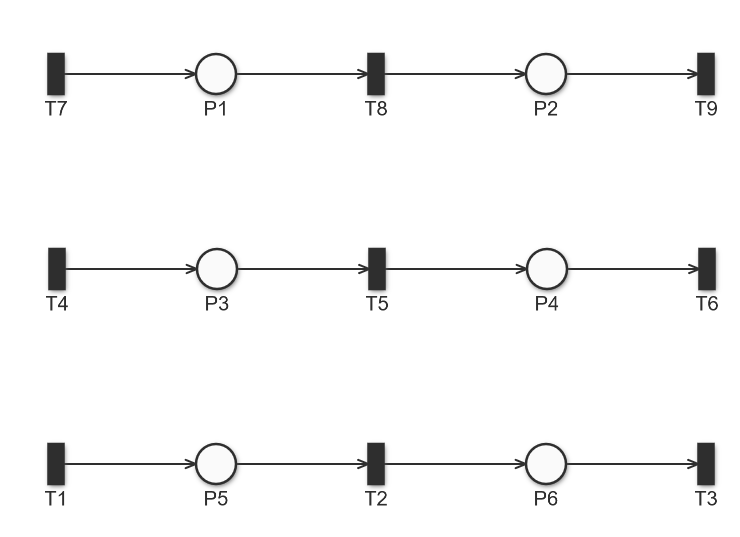
\includegraphics[width=0.7\linewidth]{imgs/Cap2_teoria/NEW_PN2_VECCHIA_MISSIONI}
    \caption{Schema di riferimento della modellazione precedente delle alternative di risorsa per una singola missione.}
    \label{fig:pn2vecchiamissioni}
\end{figure}

Ciascuna missione mantiene una sottorete con tre transizioni e due posti
interni. Le tre fasi rappresentano l'avvio, il completamento temporizzato
e il passaggio alla missione seguente oppure il rilascio della risorsa.
Le sottoreti dello stesso ordine vengono collegate in sequenza secondo
le priorità interne.

\subsection{Intra-order mission links}

Tra due missioni consecutive viene inserito un posto di collegamento che
riceve il token dalla transizione finale della precedente e lo rende
disponibile alla transizione iniziale della successiva. Il token conserva
il colore della risorsa assegnata. Il posto di collegamento rappresenta
quindi sia la precedenza sia il mantenimento della riserva operativa.

La Figura~\ref{fig:pn1nuovamissioni} mostra una sequenza di tre missioni;
i posti $P7$ e $P8$ collegano le rispettive sottoreti. Lo schema evidenzia
le precedenze e va letto insieme al vincolo sul colore della risorsa.

\begin{figure}[H]
    \centering
    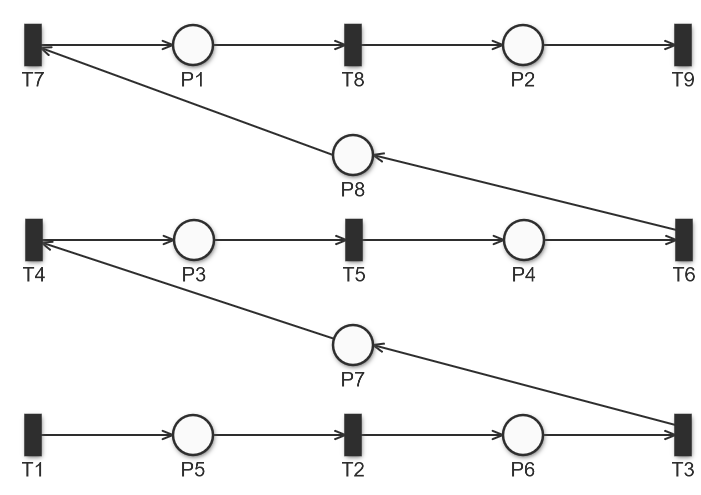
\includegraphics[width=0.7\linewidth]{imgs/Cap2_teoria/NEW_PN1_NUOVA_MISSIONI}
    \caption{Collegamento tra tre missioni dello stesso ordine mediante posti di precedenza. Il token della risorsa viene trasferito lungo la sequenza senza essere restituito al posto comune tra missioni intermedie.}
    \label{fig:pn1nuovamissioni}
\end{figure}

Solo la prima missione dell'ordine preleva il token dal posto comune delle
risorse disponibili; solo l'ultima missione ammessa lo restituisce.
All'interno dell'ordine, la disponibilità necessaria all'avvio è rappresentata
dal token nel posto di collegamento: non occorre prelevare nuovamente una
risorsa libera dal posto comune.

For each resource $r\in\mathcal R$, exactly one token of color $r$ exists in the
operational CPN. Hence, the corresponding resource token is conserved by every
transition firing. This property can be expressed as the following place invariant:

\begin{equation}
	\sum_{p\in\mathcal P} M(p)(r) = 1,
	\qquad \forall r\in\mathcal R,
\end{equation}

\noindent where $M(p)(r)$ denotes the multiplicity of color $r$ in the marking of place
$p$, and $\mathcal P$ is the set of places of the operational net.
The marking determines which transitions are enabled, whereas the
order--resource assignment restricts the resource color that can participate
in their firing.

\begin{nota}
	Per semplicità di rappresentazione, le reti di Petri mostrate nelle figure non sono CPN, bensì PN. Questo perché ciascuna figura rappresenta un singolo ramo della rete, percorso da token appartenenti a un unico colore, consentendo così una rappresentazione grafica semplificata.
\end{nota}

\subsection{Esclusione, fallimento e prosecuzione dell'ordine}

Una missione esclusa nella preparazione non genera una sottorete operativa.
Se invece una missione ammessa non dispone di un percorso valido, viene
registrata come fallita e il token viene trasferito oltre il relativo ramo,
consentendo di esaminare la missione successiva dello stesso ordine.
In questo caso non si aggiorna la posizione della risorsa e non si attribuisce
il tempo di un'esecuzione che non è avvenuta.

La riserva permane fino al termine della sequenza ammessa, anche quando
alcune missioni falliscono. Il rilascio finale della risorsa non implica
che l'ordine sia completato con successo: un ordine con missioni fallite
viene classificato come incompleto quando tutte le missioni ammesse sono
terminate. Le esclusioni preliminari, invece, non entrano nel riepilogo
delle deadline corrente e richiedono una verifica separata rispetto
all'ordine originario.

\section{Continuità dello stato tra batch}
\label{sec:progetto-tempo}

\subsection{Marcatura persistente e stato degli ordini}

La rete conserva struttura e marcatura tra batch successivi, secondo la
politica della Sezione~\ref{sec:progetto-assegnazione}. Il confine del batch
non reinizializza i token nel posto comune. Se un ordine non è concluso,
il token rimane nello stato raggiunto e mantiene il colore della risorsa
proprietaria; le missioni residue possono essere ammesse nelle code del
batch successivo rispettando le precedenze.

Sono conservati anche le posizioni delle risorse, i tempi cumulati, gli
esiti delle missioni, le associazioni ordine--risorsa e le deadline già
fissate. I contatori $C_k(t)$ e $A_k(t)$ e il lavoro $W_{r,k}(t)$ riguardano
invece il batch corrente. L'ammissione in coda e l'abilitazione nella rete
sono condizioni distinte: una missione viene eseguita quando è stata
ammessa e le precedenze e la disponibilità del token ne consentono l'avvio.

\subsection{Avanzamento temporale e rifornimento delle code}

L'avanzamento tra eventi riprende il principio della Scheduled Event List
descritto nella Sezione~\ref{sec:theory-sel}; la politica di ammissione
stabilisce quali missioni possono entrare nel processo di esecuzione.

Per una missione pianificata con successo e avviata all'istante $s_m$,
il completamento è $c_m=s_m+\tau_m$. Il motore avanza tra gli eventi
delle missioni concorrenti e aggiorna lo stato all'istante corrispondente.
Se una risorsa conserva missioni nella propria coda, può proseguirne
l'esecuzione senza richiamare lo scheduler. Quando la coda si esaurisce,
il rifornimento avviene se rimangono posti nel target e lavoro assegnabile.
Anche un fallimento può liberare un posto e richiedere un nuovo intervento.

Le code ancora attive restano invariate. Le nuove code rispettano i limiti
$q_{\max}$ e $h_q$ e il vincolo $C_k(t)+A_k(t)\leq x$; le stime ripartono
dalle posizioni effettive correnti. Le risorse eseguono in parallelo le
missioni ammesse, pur potendo accumulare attese dovute a compatibilità,
proprietà e distribuzione del lavoro.

Il batch termina al raggiungimento del target oppure quando il lavoro
pendente è esaurito e tutti i tentativi ammessi sono terminati. Il suo
istante finale è $F_k=\max_r f_{r,k}$ e, se rimane lavoro, il successivo
batch inizia a $t_{k+1}=F_k$. La deadline comune $D_k=t_k+H$ non introduce
un'attesa obbligatoria né un arresto: un batch può terminare prima o dopo
questo riferimento. Gli interventi di assegnazione seguono l'esaurimento
delle code e la disponibilità di posti, anziché un controllo periodico.

\subsection{Missioni fallite e prosecuzione tra batch}

Una missione senza percorso valido è registrata come fallita senza
incrementare il tempo di lavoro né aggiornare la posizione. Il token
prosegue verso la missione successiva dell'ordine o verso il rilascio finale.
Il fallimento riduce $A_k(t)$ senza incrementare $C_k(t)$: il posto liberato
può essere occupato da altro lavoro, mentre l'esito della missione fallita
rimane registrato. Un ordine con almeno una missione fallita risulta
incompleto quando tutte le sue missioni ammesse sono terminali.

Le missioni residue di un ordine al confine tra batch rappresentano lavoro
da proseguire sulla stessa risorsa. Non costituiscono, da sole, un'anomalia
né comportano una nuova assegnazione del proprietario. Se il lavoro
eseguibile si esaurisce prima del target, il riepilogo registra i
completamenti mancanti. Le esclusioni preliminari restano separate dagli
esiti delle missioni ammesse e dal monitoraggio delle deadline.

\section{Stima euclidea delle deadline}
\label{sec:stima-deadline-manhattan}

La costruzione delle scadenze applica le definizioni della
Sezione~\ref{sec:theory-deadlines}. Qui vengono precisati i parametri,
il trattamento delle coordinate e il congelamento delle previsioni.

Le deadline degli ordini sono ricavate dalla geometria delle missioni.
Il tempo nominale $\overline{\tau}=180\,\mathrm{s}$ serve invece a definire
il budget del batch $H$ e l'orizzonte delle code $h_q$, come descritto nella
Sezione~\ref{sec:progetto-assegnazione}. La deadline comune $D_k$ e le
deadline dei singoli ordini hanno quindi origini e ambiti diversi.
Il tempo nominale non sostituisce le durate calcolate mediante A* o le
previsioni euclidee dei singoli ordini.

La deadline viene fissata al primo avvio di una missione dell'ordine per cui
la pianificazione ha avuto successo. Non decorre dall'assegnazione alla risorsa:
il tempo impiegato dalla risorsa negli ordini precedenti non consuma il
budget del nuovo ordine. Le scadenze sono indicatori osservativi e non
impediscono l'avvio né interrompono missioni in ritardo.

\subsection{Sequenza e distanza stimata}

Sia $\pi_o=(m_{o,1},\ldots,m_{o,n_o^{\mathrm{amm}}})$ la sequenza delle
missioni ammesse dell'ordine, ordinata per priorità decrescente e, a parità,
per ordine di ingresso. La previsione comprende tutte queste missioni,
anche se una precedente missione della sequenza è già fallita prima del
primo avvio riuscito. Le missioni escluse in preparazione non sono incluse.

Gli estremi $F_i$ e $T_i$ sono espressi negli indici della griglia dopo
normalizzazione e arrotondamento, rispettivamente FROM e TO. La stima non esegue A* e non applica le
correzioni degli estremi occupati o non raggiungibili adottate dal planner.
Usa la distanza euclidea
\begin{equation}
    d_E(p,q)=\sqrt{(x_p-x_q)^2+(y_p-y_q)^2}.
    \label{eq:manhattan-distance}
\end{equation}
Indicando con $P_r$ la posizione corrente della risorsa prima del primo
avvio riuscito, si pone $Q_1=P_r$ e $Q_i=T_{i-1}$ per $i>1$. Quando la
risorsa non ha una posizione precedente, si assume $Q_1=F_1$. Per ogni
missione la distanza prevista è
\begin{equation}
    \widehat\ell_{o,i}=d_E(Q_i,F_i)+d_E(F_i,T_i).
    \label{eq:estimated-order-distance}
\end{equation}
Sono così considerati l'avvicinamento iniziale, le movimentazioni FROM--TO
e i trasferimenti tra missioni consecutive. Non si aggregano prelievi o
consegne anche quando più missioni condividono la destinazione.

Con $v_c=5.5$ celle al secondo, maggiorazione $\alpha=0.20$, contributo
accessorio $\tau_f=60\,\mathrm{s}$ e margine per missione $\delta_m$, si ha
\begin{equation}
    \widehat\tau_{o,i}=
    \operatorname{round}\!\left(
       \frac{\widehat\ell_{o,i}}{v_c}(1+\alpha)\right)
       +\tau_f+\delta_m,
    \qquad \delta_m=0\,\mathrm{s}.
    \label{eq:stima_scadenze}
\end{equation}
L'arrotondamento viene applicato separatamente a ciascuna missione, prima
della somma. La durata stimata dell'ordine è
\begin{equation}
    \widehat D_o=\sum_{i=1}^{n_o^{\mathrm{amm}}}\widehat\tau_{o,i}.
    \label{eq:estimated-order-duration}
\end{equation}
Il margine configurabile si applica a ogni missione: non è un termine unico
per ordine e non dipende automaticamente dal numero di coordinate rimappate.

Sia $S_o$ il primo avvio riuscito dell'ordine. Le deadline delle missioni
sono cumulative e la deadline dell'ordine coincide con l'ultima:
\begin{equation}
    d_{o,i}=S_o+\sum_{j=1}^{i}\widehat\tau_{o,j},
    \qquad d_o=S_o+\widehat D_o.
    \label{eq:estimated-order-deadline}
\end{equation}
Tutte le previsioni dell'ordine vengono congelate insieme comportanto che le missioni
successive e il passaggio tra batch non vengono ricalcolate. Se nessuna missione
dell'ordine viene pianificata con successo, avvio e deadline restano
indefiniti quindi un ordine con sole missioni fallite risulta incompleto.


\subsubsection{Separazione dal path planning}
La previsione congelata per le deadline non modifica il planner A*,
la possibilità di movimenti diagonali o l'abilitazione delle transizioni.
Lo scheduler usa inoltre stime euclidee aggiornate per dimensionare e
bilanciare le code brevi: queste stime dipendono dalle posizioni correnti
e non ricalcolano le deadline degli ordini. La durata simulata dipende dal
numero di punti del percorso pianificato, mentre la previsione usa distanze
euclidee tra gli estremi richiesti. Pur condividendo i coefficienti temporali,
le due procedure non misurano la stessa quantità geometrica.


\subsection{Slack e ritardo}

Gli indicatori riprendono le definizioni delle
Equazioni~\ref{eq:order-slack} e~\ref{eq:order-tardiness}, applicandole
sia alle singole missioni sia agli ordini completati. Per una missione completata all'istante $c_{o,i}$ si definiscono
\begin{equation}
    \sigma_{o,i}=d_{o,i}-c_{o,i},\qquad
    T_{o,i}=\max\{0,c_{o,i}-d_{o,i}\}.
\end{equation}
Per un ordine le cui missioni ammesse sono tutte completate, con istante
finale $C_o$, valgono analogamente
\begin{equation}
    \sigma_o=d_o-C_o,\qquad T_o=\max\{0,C_o-d_o\}.
\end{equation}
Uno slack positivo indica \textit{anticipo} mentre uno negativo indica \textit{ritardo}.
Il ritardo positivo, o \textit{tardiness}, è distinto dalla
\textit{lateness} con segno $C_o-d_o$. Una missione può superare la propria
scadenza cumulativa senza che l'ordine termini necessariamente in ritardo,
se le attività successive recuperano il tempo. Lo stato corrente calcola
questi indicatori sui completamenti; non aggiorna un ritardo corrente degli
ordini aperti mediante un orologio a finestre.

\subsubsection{Prediction limits}
Obstacles, path deviations, outer points corrections, tiles counting and roundings may produce 
deviations.
Ostacoli, deviazioni di percorso, correzioni degli estremi, conteggio dei punti e
arrotondamenti possono produrre scostamenti. La durata prevista non va
interpretata come una garanzia né come un limite inferiore o superiore
universale della durata simulata. La correzione delle coordinate esterne
alla mappa non ricostruisce il tempo di percorrenza fuori dal dominio. Da sottolineare
che il comportamento umano comporta sempre un fattore stocastico di cui non 
si può tenere conto se non introducendo ulteriori fattori di compensazioni temporali (come $\delta_m$ in \ref{eq:stima_scadenze}).




